\chapter{相关工作}
本章将对本文的研究框架中所涉及的相关技术进行分析,主要分为三个方面:一个方面是介绍结构图表征的相关算法,也就是单纯对网络的结构进行表征学习的相关技术及其发展演化,第二是对属性网络中相关的图表征算法进行介绍和分析,第三是对增量学习相关的技术细节进行分析。



%%%%%%%%%%%%%%%%%%%%%%%%%%%%%%%%%%%%%%%
%------------------------------------     结构图表征算法     -------------------------------------%
%%%%%%%%%%%%%%%%%%%%%%%%%%%%%%%%%%%%%%%
\section{结构图表征算法}
图表征(Network Embedding/Representation)过程是通过一定算法获得网络中所有节点向量表征的一个过程,这类算法本身类似于一个完整任务的中间流程,因为没有对应的量化指标去直接衡量图表征算法是否性能突出,图表征算法从某些程度类似于高维数据的降维过程,降维之后需要放入特定的机器学习任务,如节点分类、节点聚类(社区发现)、节点相似度计算、链路预测等,通过学习任务的指标来衡量图表征过程的优良。虽然没有一个公认的量化指标来对图表征算法性能进行评价\cite{goyal2017graph},但是在设计图表征算法的时候需要考虑一些准则来达到利于数据可视化或者后续学习任务的目的,一般而言需要考虑以下几点:
\begin{itemize}
	\item { 对网络性质的保留:有效合理的图表征向量需要能够保留下网络本身的结构特征,比如节点间因为连接而产生的相似度,在向量化表征之后可以得到近似的结果。在这一方面存在的难题是,网络本身的性质存在很多,比如相似度、距离,这些性质在表征向量中不一定能完全兼顾,因此对于不同的图表征算法,其性能好坏取决于后续的具体应用。}
	\item {伸缩性:现实应用中的网络规模非常巨大,大型网络中节点至少都是千万级别的,节点间的连边的量级更是十亿级别的,所以图表征算法的可扩展性是非常具有现实意义的,但是当需要设计一个能保留网络全局信息的图表征算法的时候,设计一个伸缩性性好的算法是非常具有挑战性的。}
	\item {表征向量的维数:对于表征向量来说,挑选一个合适的向量维度是比较困难的。高维向量会保留更多的网络原本的信息,从直观上理解,就相当于减小了舍入误差,但是过高维的向量表征对于学习任务来说其复杂度是不友好的;低维向量表征虽然能优化计算复杂度,但是过低维的向量表征会丢失一部分精度。对于向量表征的维度也是根据学习任务的不同特点来调整的。}
	\item {自适应性:对于大型网络来说,做一次向量表征的计算成本是比较高的,在大型网络中不可忽略的是网络一直在变化演进中,包括网络的结构信息,如新增节点和连边的增删等,还有节点的属性信息都是时刻在变动的,从计算资源和学习任务时效性来讲,新的网络信息不应该重复地进行同样的学习过程,好的网络表征算法应该考虑到网络的动态变化。}
\end{itemize}

\textbf{图表征算法的定义}:给定一个图$G = (V,E)$,$V$表示网络$G$中节点的集合,$E$表示网络$G$中连边的集合,通常图是用邻接矩阵$A \in R^{|V|\times|V|}$表示的,图表征算法的定义就是通过寻找一个映射函数来表征网络中的每个节点:
\begin{equation}
f_G: A \rightarrow R^{|V| \times d} \qquad s.t.\quad d<<|V|
\end{equation}

\begin{figure}
	\centering
	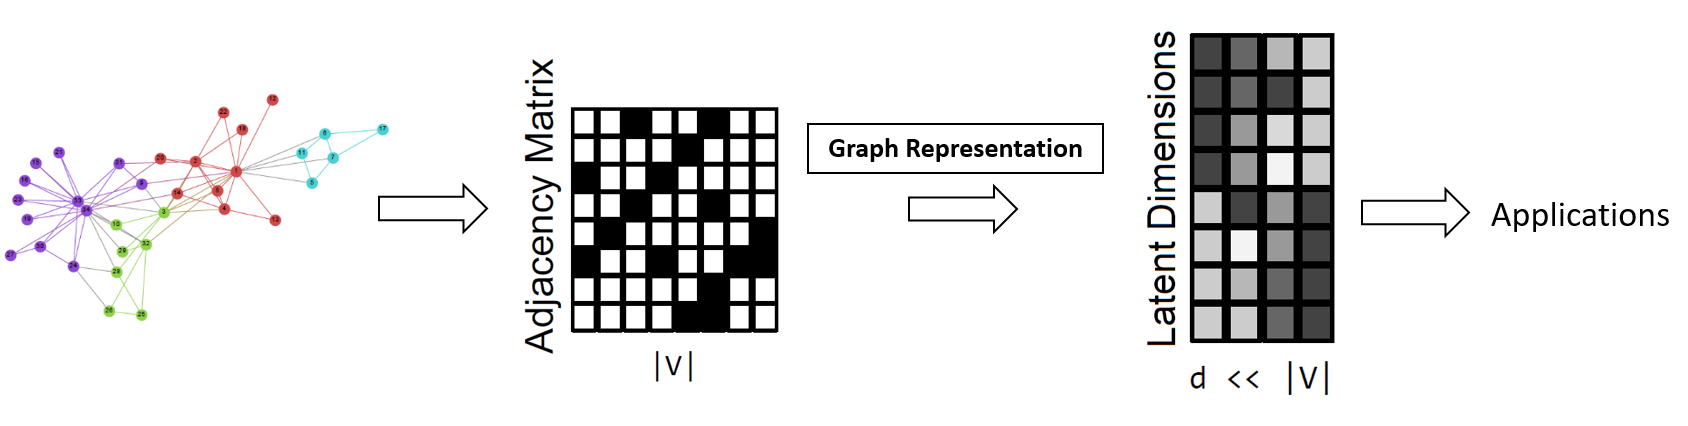
\includegraphics[width=5.5in]{figures/network_embedding}
	\caption{图表征算法}
\end{figure}


网络的邻接矩阵随着图中节点规模的增大,会变得非常稀疏,也就显现出了低秩的性质。对于低秩矩阵的流形学习的思想类似于图表征的过程。流形学习(Manifold Learning)领域提出借鉴拓扑流形的降维方式,这些方法通过设计一些表示节点间关系的矩阵,通过特征值分解的方法来获得表征向量,比如最基础的用来表示节点之间关系的邻接矩阵$A$,拉普拉斯矩阵 $L$(Laplacian Matrix)。通过分析,适用特征值分解的方式,需要矩阵满足对称正定,对于设计不符合要求的矩阵则需要根据随机梯度下降(Stochastic Gradient Descent)去求解。
在2013年,Google的开源工具Word2Vec\cite{mikolov2013efficient}发布之后,借鉴词向量表征的思路,Node2Vec和DeepWalk算法以蒙特卡罗随机游走的方式进行网络路径采样,将采样得到的路径视为词向量表征中的语料库,然后采用类似Word2Vec方法进行学习。在2015年,Jian Tang\cite{tang2015line}在提出LINE算法的同时提出了接近度的概念,根据接近度的概念,可以将不同的图表征算法进行分类。下面主要介绍一下接近度的概念,然后基于接近度的阶数,按从低阶到高阶接近度依次介绍:%局部线性嵌入LLE(Locally Linear Embedding),%
拉普拉斯映射LE(Laplacian Eignemaps) , LINE(Large-scale Information Network Embedding)算法,Node2Vec算法。% DeepWalk算法,。
\subsection{接近度}
\definition{\textbf{一阶接近度}:}\label{first_order}
网络中的一阶接近度是用来描述节点对的局部接近特性。在网络$G$中,对于有连边的节点对($u$,$v$)
连边的权重$A_{uv}$则为一阶接近度(first-order proximity),对于没有连边的节点对,则一阶接近度则为0。

所谓一阶接近度,通常是用来描述网络中直接相连节点对之间的相似度,直观的理解可以视为一阶接近度用来描述网络的一度邻居结构,也即局部结构,这也是符合常识和具体的应用场景的,例如在社交网络中,有直接联系的节点往往具有更强的亲密度。在获取和交换信息上,用户节点更加倾向于直接作用给一度邻居。基于这一点构想,很多算法基于保留一阶接近度的方法来构造目标函数,然后通过优化目标函数得到所求的表征向量,其中包含IsoMap算法,局部线性嵌入算法,拉普拉斯特征映射算法,图分解GF\cite{ahmed2013distributed}(Graph  Factorization)。

但在现实的网络场景中,一阶接近度是存在局限性的。局限性来源于两方面:第一方面来自于数据收集的问题,收集到的网络数据未必能完全体现物理世界中真实的全部连接数据\cite{liben2007link} ,一些存在直接链接的节点可能在数据收集过程丢失,这种缺失情况在只保留一阶接近度的情况下是存在局限的。第二方面,网络本身的特性使得网络存在路径,节点对之间的路径往往不唯一,用来表示非直接连接节点对之间的相似度一般用最短距离来描述,这种情况对于只保留一阶接近度的图表征来说是很难解决的,从而会损失掉一部分网络的信息;因此在图表征算法中只采用保留一阶接近度的方式对于很好地保留网络的信息是不够的,也就是需要引入高阶接近度来描述网络结构本身。保留高阶接近度的含义是保留一些非直接联系但是因为网络连接而具备较大可能产生连接,比如,在社交网络中有较多共同邻居或者同属于一个社区中的节点对更有可能会产生连边。下面介绍一下高阶接近度中的一个特例:二阶接近度。

\definition{\textbf{二阶接近度}:}\label{second_order}
网络中的二阶接近度是用来描述节点对各自周边节点环境的相似度。也就是说,节点$u$和节点$v$的二阶接近度取决于各自的邻居节点集合$N(u)$和$N(v)$,如果$|N(u) \cap N(v)|>0$,也即节点$u$和节点$v$有共同邻居,则二阶接近度大于0;否则,二阶接近度等于0。

二阶接近度相比于一阶接近度保留了节点对之间邻居节点的相似度相似度信息,因此对网络结构本身保留了更多的信息,但是这也带来了复杂度显著提升的效果,在解决复杂度的问题上,一般采用文献\cite{mikolov2013distributed}中提到的负采样方法来进行效率提升。除了二阶接近度以外,DeepWalk和Node2vec采用蒙特卡罗随机游走的方式,保留网络中的路径属性,相当于可以控制游走步长而保留网络中k阶接近度,除此之外还有通过其他相似度而设计的准则来保留网络中的高阶接近度\cite{ou2016asymmetric}。

在介绍图表征算法之前先对后面用到的符号及含义进行统一定义。
\begin{table}
	\centering
	\caption{字符及其代表含义}
	\begin{tabular}{|C{1.8in}|C{3.3in}|}
		\hline
		\textbf{字符} & \textbf{含义} \\ \hline\hline
		$G$ & 网络型数据 \\ \hline
		$E$ & 网络中边的集合 \\ \hline
		$V$& 网络中点的集合 \\ \hline
		$k$ & 节点向量表征的维数  \\ \hline
		$X$ & 节点向量表征矩阵 \\ \hline
		$X_i$ & 节点i的表征向量 \\ \hline
		$A$ & 网络的邻接矩阵 \\ \hline
		$D$ & 对角线元素为节点度的对角矩阵\\ \hline
		$L$ & 网络的拉普拉斯矩阵,$L=D-W$ \\ \hline
		$S$ & 网络节点的相似度矩阵 \\ \hline
		$B^T$ & 某个矩阵B的转置 \\ \hline
		$tr(B)$ & 某个矩阵B的迹 \\ \hline
		$I$ & 单位矩阵 \\ \hline
	\end{tabular}
\end{table}

\subsection{拉普拉斯特征映射(Laplacian Eigenmaps)算法}
首先,基于前面介绍的接近度概念,拉普拉斯特征映射采用的是保留一阶接近度的思想,该算法假设两个节点$i$和$j$之间的连边权重$A_{ij}$越大,则对应地它们的表征向量的差距应该越小,在该算法中以表征向量差的二范数来表征这个差距,也就是需要最小化如下的目标函数:
\begin{equation}
\begin{aligned}
\phi(X) &= \frac{1}{2}\sum_{i,j}|X_i - X_j|^2A_{ij} \\
&= \frac{1}{2}(\sum_{i,j}(x_i^2+x_j^2-2x_ix_j) A_{ij}) \\
&=\frac{1}{2} (\sum_ix_i^2D_{ii} +\sum_j x_j^2 D_{jj} - 2\sum_{i,j}x_i x_j A_{ij}) \\
&= tr(X^TLX)
\end{aligned}
\end{equation}
为了得到合理的解,原优化问题需要增加约束$X^TDX=I$,通过添加约束去掉平凡解。原优化问题变成:
\begin{equation}
\min_{X^TDX} \quad tr(X^TLX)
\end{equation}
对约束条件进行利用,优化表达式,令$X=D^{-\frac{1}{2}}U$,代入约束条件中可证明正确性。于是问题原来的优化问题转化成如下的带约束优化的优化问题:
\begin{equation}\label{laplacian_reduce}
\begin{aligned}
\min_{U^TU = I} &\quad tr(U^TD^{-\frac{1}{2}}LD^{-\frac{1}{2}}U) \\
&= tr(U^T(I-D^{-\frac{1}{2}}AD^{-\frac{1}{2}})U)
\end{aligned}
\end{equation}
于是可以将原问题进一步转变成一个求最大值的优化问题:
\begin{equation}
\max_{U^TU = I} tr(U^TWU)
\end{equation}
其中$W = D^{-\frac{1}{2}}AD^{-\frac{1}{2}} $,于是问题转化为求解$W$矩阵的前k个最大特征值所对应的特征向量,通过特征值分解可以得到特征值及对应的特征向量,前k个特征向量组合成的$|V|\times k$矩阵就是最后的节点表征矩阵。

\subsection{LINE算法}
 \begin{figure}[!ht]
	\centering
	{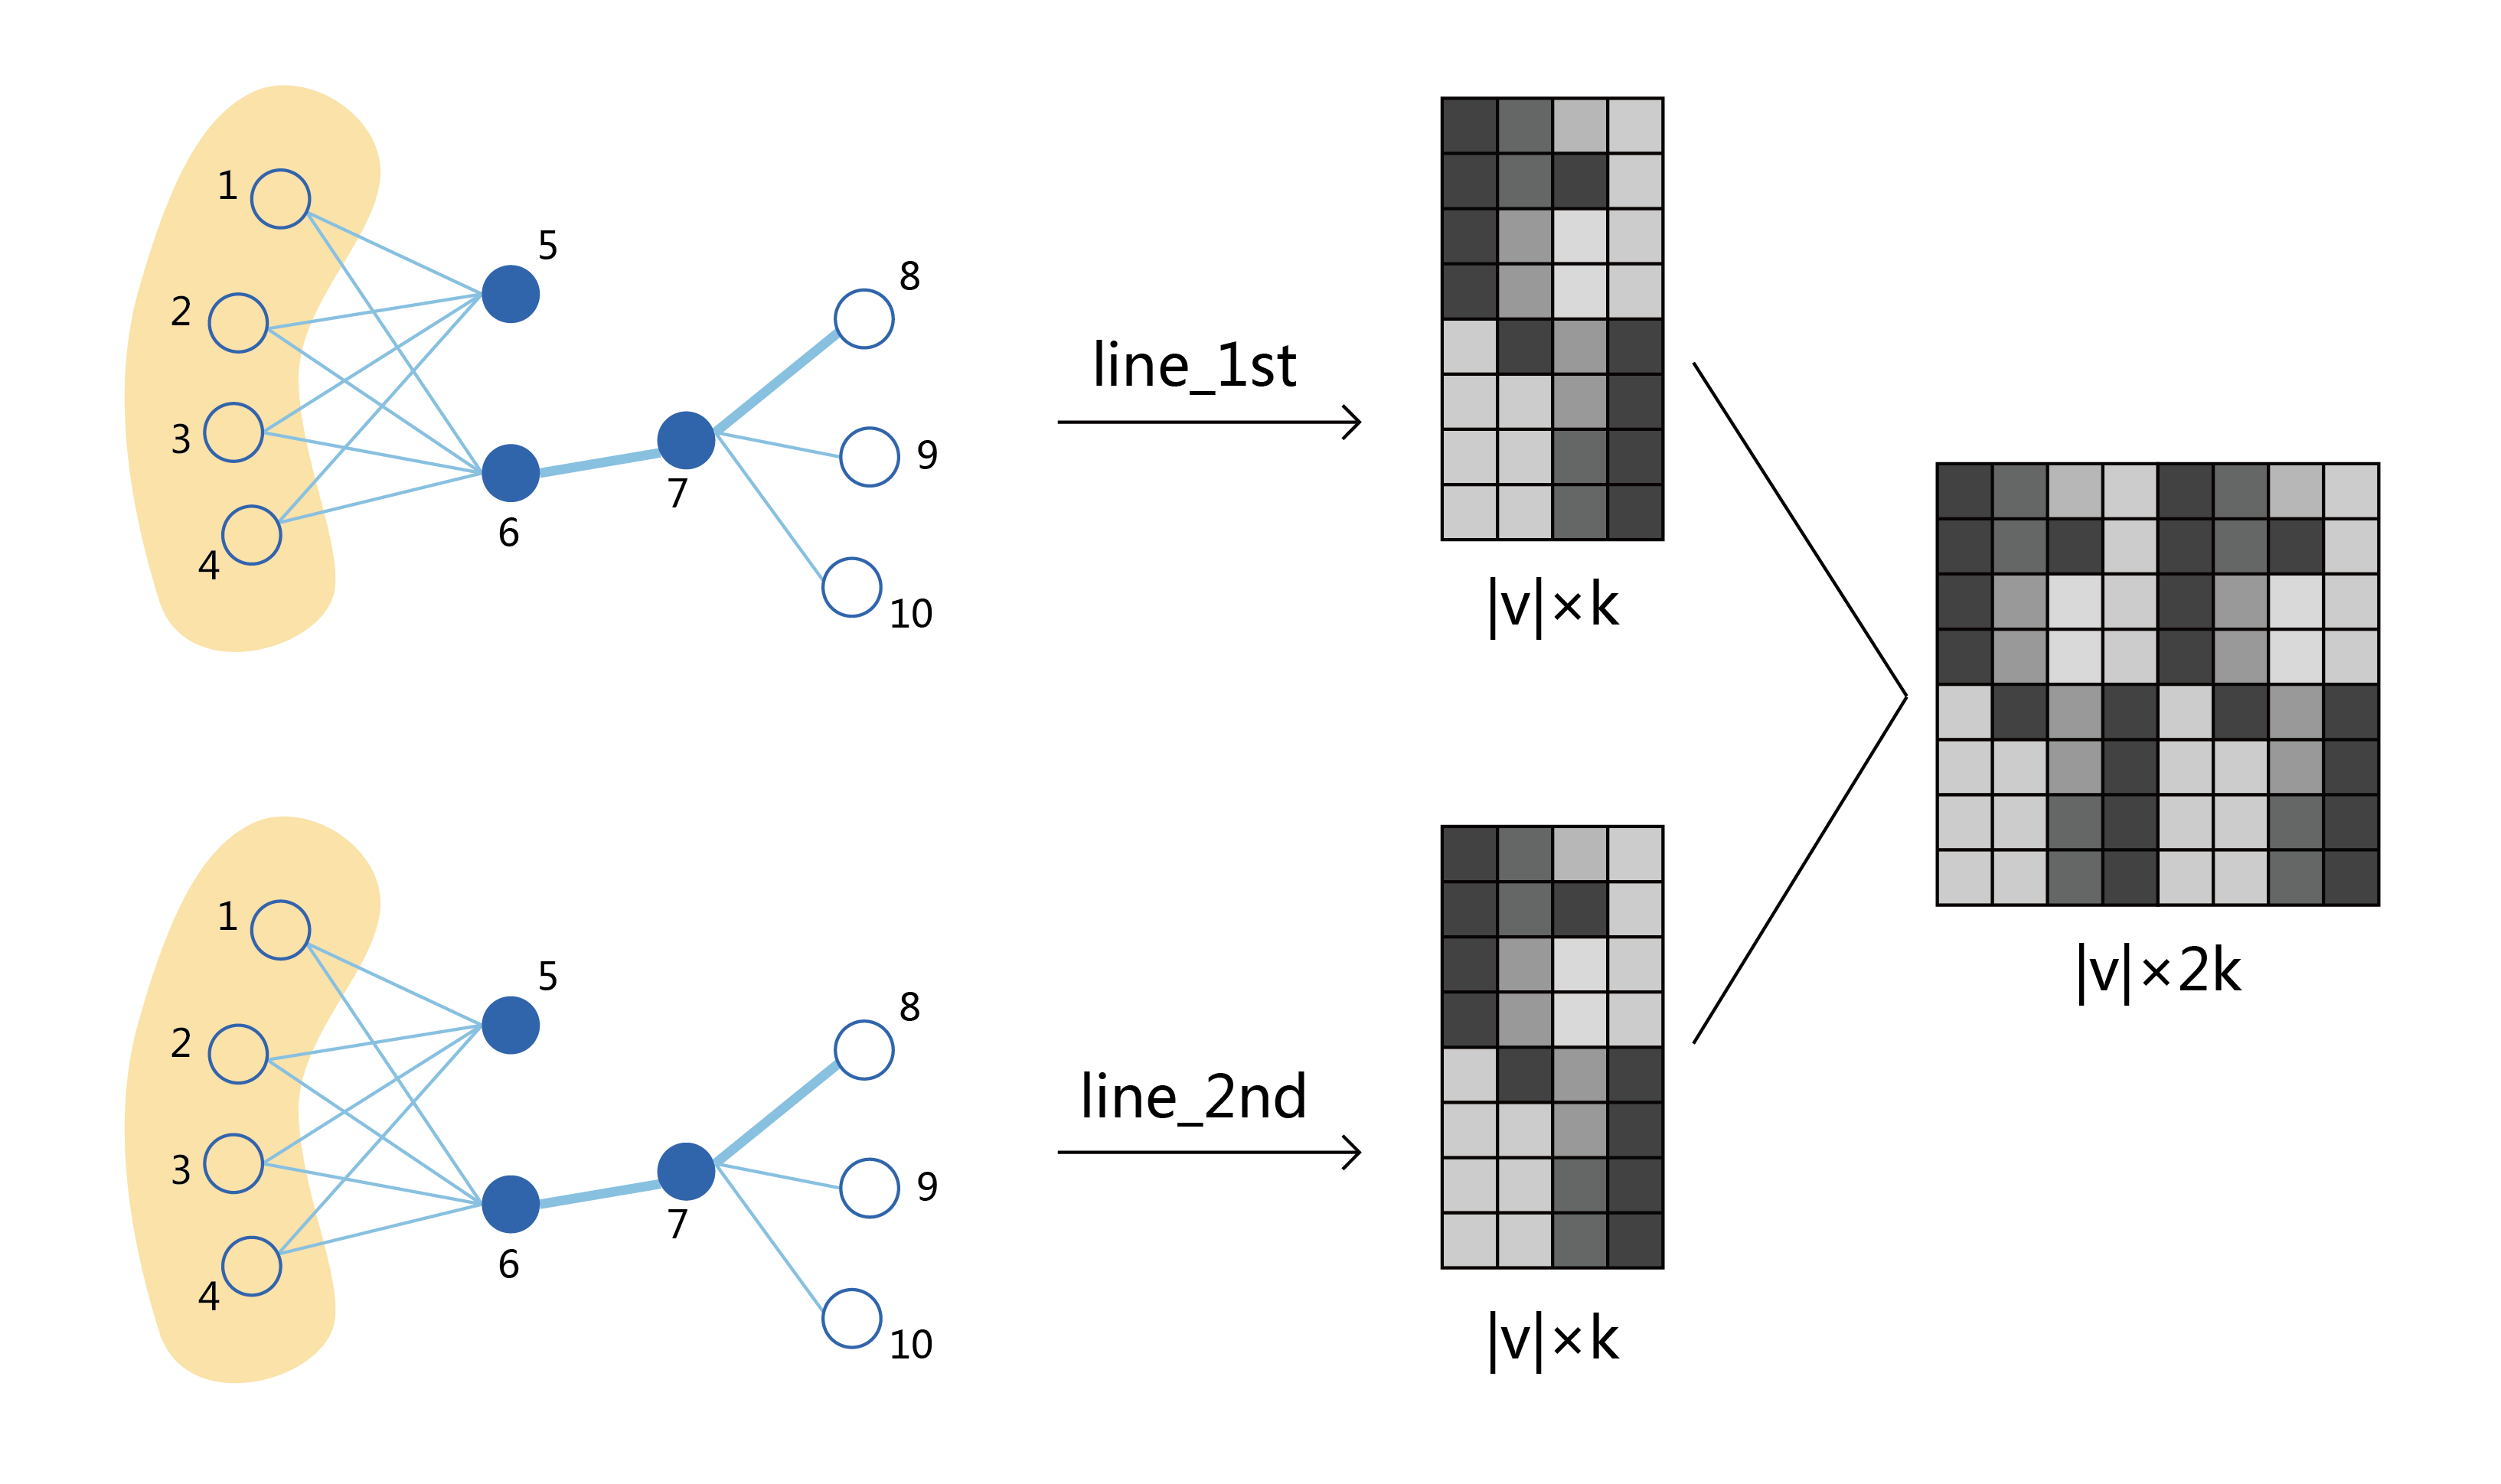
\includegraphics[width=5in]{figures/line.png}}
	\caption{line的算法流程:一阶接近度需要保证节点6,7的表征向量比较接近;二阶接近度保证拥有较多共同邻居的节点5和节点6的表征向量比较接近}\label{line_process}
\end{figure}
 不同于前面的拉普拉斯特征映射,LINE算法设计成保留一阶接近度和二阶接近度的方式,该算法在设计保留节点$i$和节点$j$之间一阶接近度时,首先定义节点$i,j$的联合概率为:
 \begin{equation}
 p_1(i,j) = \frac{1}{1+exp(-X_i^T \cdot X_j)}
 \end{equation}
 将联合概率推至网络整体,得到整个网络中所有有连边的节点对之间的联合概率集合$p_1(\cdot,\cdot)$。根据之前的定义,一阶接近度为网络中连边的权重,作者在这里首先将连边权重进行规范化,即令$A_{ij} =A_{ij}/\sum_{i,j}A_{ij} $,规范化后的连边权重作为一阶接近度,并将对应值记为经验联合概率$\hat{p}_1(\cdot,\cdot)$。该算法中假设联合概率集合$p_1(\cdot,\cdot)$应尽量接近于一阶接近度$\hat{p}_1(\cdot,\cdot)$,为衡量两个集合$p_1(\cdot, \cdot)$和$\hat{p}_1(\cdot,\cdot)$的接近程度,文中引入KL散度来作为距离函数。因此为保留一阶接近度设计的目标函数为:
 \begin{equation}
 	\min KL(\hat{p}_1(\cdot, \cdot),p_1(\cdot,\cdot))
 \end{equation}
 其中$KL(p,q) = \sum_{i=1}^{n}p(x)\log\frac{p(x)}{q(x)}$,代入上式,去掉常数量对目标函数进行化简得到:
 \begin{equation}\label{line_1st}
 	\min -\sum_{(i,j) \in E} A_{ij}\log p_1(i,j)
 \end{equation}
 通过异步随机梯度下降对目标函数进行优化,得到保留一阶接近度的表征向量。
 
 为保留二阶接近度,论文中假设节点$i$存在两种向量表征,一种是节点$i$为当前观察节点时的向量表征$X_i$,一种是该节点为其他节点的上下文环境时的向量表征$X'_i$,并以此定义一个条件概率$p_2(j|i)$,用来表示当前观察节点为$i$时,节点$j$的概率:
 \begin{equation}
 	p_2(j|i) = \frac{\exp(X\prime_j^T \cdot X_i)}{\sum_{k=1}^{|V|}\exp(X\prime_k^T \cdot X_i)}
 \end{equation}
 
 对于单个节点$i$,$p_2(\cdot|i)$表示所有节点为其上下文(邻居节点)概率的集合。根据二阶接近度的定义,保留二阶接近度即保留其邻居节点的分布,在文中将二阶接近度设为按节点出度规范化之后的连边权重,同时定义二阶接近度为当前节点的经验条件概率集合$\hat{p}_2(\cdot|i)$,有$\hat{p}_2(\cdot|i) = \frac{W_{ij}}{d_i}$,其中$d_i$表示节点$i$的出度。则根据假设需要优化$p_2(\cdot|i)$和$\hat{p}_2(\cdot|i)$的距离函数,则为保留二阶接近度的目标函数形式如下:
 \begin{equation}
 \min \sum_{i \in V}\lambda_i KL(\hat{p}_2(\cdot|i),p_2(\cdot|i))
 \end{equation}
 其中$\lambda_i$用来对不同的节点进行加权,表示节点在网络中的重要性,可以通过节点度或者PageRank\cite{page1999pagerank}值来衡量,在文中采用节点度的形式,也即令$\lambda_i=d_i$。将KL散度表达式代入上式,去掉常数量化简,得到保留二阶接近度的目标函数:
 \begin{equation}\label{line_2nd}
 \min -\sum_{(i,j) \in E} A_{ij}\log p_2(j|i)
 \end{equation}
 优化方式仍采用异步随机梯度下降,得到保留二阶接近度的表征向量。从表达式可以看出优化计算二阶接近度时的复杂度比较高,文中采用负采样的方式对目标函数进行优化,从而降低了计算复杂度。另外,文中保留一阶接近度和二阶接近度的方法采用比较直接的合并方式,也即将优化式(\ref{line_1st})得到的表征向量和优化式(\ref{line_2nd})得到的表征向量直接并排合并起来,作为新的表征向量,如图\ref{line_process}所示。通过实验,LINE算法在可视化和文档分类应用上有很好的效果。

\subsection{DeepWalk算法}
DeepWalk算法通过统计,论证网络的无标度特性与语料库中单词的幂律分布之间的联系,采用随机游走的方式进行路径抽样产生标准的输入序列,并通过语言模型来进行图向量表征。语言模型的功能是去评估特定单词序列在语料库中出现的概率,为此需要通过训练语料库最大化单词序列的概率。也即,给定单词序列$W = (\omega_0, \omega_1,\cdots,\omega_n)$,需要最大化条件概率$p(\omega_n |\omega_0,\omega_1,\cdots,\omega_{n-1})$,文中通过随机游走采样的短路径类比于单词序列,假设采样到的一条短路径为$V = (v_1, v_2, \cdots, \v_n)$,则需要最大化的条件概率为:
\begin{equation}
	p(v_n | v_0, v_1,\cdots,v_{n-1})
\end{equation}
在Word2Vec语言模型中,最大化条件概率为目标函数,但是同时需要得到词向量表征这个中间结果。于是问题变成:需要寻找一个表征函数$\Phi:v\in V \rightarrow R^{|V|\times d}$对词进行向量表征,并将表征向量作为输入调整目标条件概率。类比在网络中的场景,目标条件概率形式变成:
\begin{equation}\label{deepwalk_1}
	p(v_n | \Phi(v_0), \Phi(v_1),\cdots,\Phi(v_{n-1})) 
\end{equation}
从式(\ref{deepwalk_1})中可以看出,当游走路径长度$n$变大时,概率计算难度变大。在Word2Vec算法中,根据不同场景设计两种模型CROW(Continuous Bag-of-Words Model)和Skip-gram(Continuous Skip-gram Model)。CROW模型是已知单词$\omega_i$上下文单词序列,最优化单词$\omega_i$的概率,与之相反,Skip-gram模型则是采用已知单词$\omega_i$,最优化上下文单词序列的概率。在DeepWalk中,采用Skip-gram模型,以短路径类比单词序列,设定路径长度为$2l$,则需优化的目标函数为:
\begin{equation}
\begin{aligned}
	\min_{\Phi} &-\log p(v_{i-l},\cdots,v_{i-1},v_{i+1},\cdots,v_{i+l}| \Phi(v_i)) \\
	&= \prod_{j=i-l,j\neq i}^{i+w} p(v_j|\Phi(v_i))
\end{aligned}
\end{equation}
其中根据独立条件假设对目标函数进行简化。DeepWalk采用分层softmax(Hierarchical Softmax)的方式来求解上述目标函数,构建一个Huffman树,其中每一个非叶子节点视为一个二分类的分类器,将每一个$p(v_j|\Phi(v_i))$视为叶子节点,其值等于从根节点到到叶子节点的路径所有非叶子节点的概率值累乘,通过随机梯度下降的方式优化目标函数。DeepWalk算法在真实数据上的节点多标签分类实验表现很好。
\begin{figure}[!ht]
	\centering
	{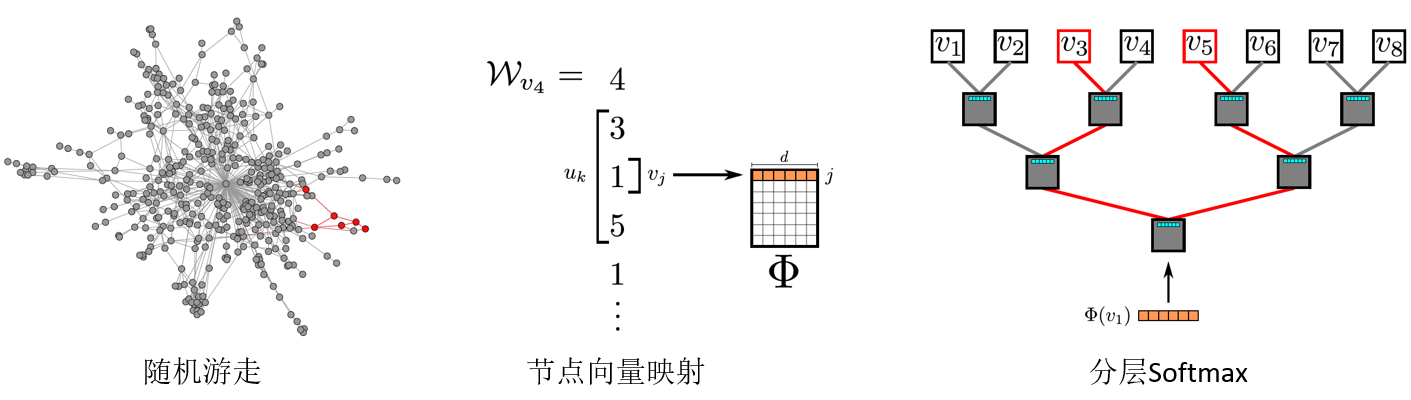
\includegraphics[width=6in]{figures/deepwalk2.png}}
	\caption{DeepWalk的算法流程}\label{img2.5}
\end{figure}

通过对比DeepWalk,LINE,LE的算法思想,可以看出基于随机游走的DeepWalk保留了网络中的高阶接近度,当序列长度为$2l+1$时,即保留网络中$1-l$阶接近度,而且有不错的时间效率。
%%%%%%%%%%%%%%%%%%%%%%%%%%%%%%%%%%%%%%%
%---------------------------------------     属性网络图表征算法     ----------------------------------------%
%%%%%%%%%%%%%%%%%%%%%%%%%%%%%%%%%%%%%%%
\section{属性网络图表征}
单纯基于结构的图表征算法在很多应用都表现出较好的性能,比如文本分类、链路预测等,但是真实应用场景下的网络中,节点往往包含着丰富的属性信息。比如在论文合作网络中,除了连接紧密或者处于相同社区的研究人员会合作,在研究内容上一致或接近的研究人员也比较有可能会产生合作,也就是说,合作网络中研究人员的研究内容属性会影响链路预测的结果;对于类似维基百科的富文本网络,每个节点代表一篇文章,这些文章的内容、主题都可以作为描述这个节点的特征,而成为表征向量的一部分。比较朴素的方法是将结构表征向量和节点属性特征直接并起来作为新的表征向量,这种方式没有利用好结构和属性特征之间的联系,在\cite{li2017attributed}中则采用相对优化的投影融合的方式进行结合。更加有明显结合意义的方法是在图表征的学习框架中嵌入节点属性信息同时进行优化学习。下面主要介绍其中一种算法TADW(Text-Associated DeepWalk)算法,该算法解决的问题是有大量文本信息的图表征问题。

\subsection{TADW算法}
TADW算法是基于DeepWalk算法的改进方法,首先文中先提出并证明了DeepWalk算法与特定矩阵分解是等价的:设矩阵$M\in R^{|V|\times |V|}$,其中$M_{ij}$用来表示在固定游走步长时从节点$i$到节点$j$的对数平均概率,对矩阵$M$进行正则化低秩矩阵分解\cite{yu2014large},得到矩阵$W^T \in R^{|V| \times k}$和矩阵$H \in R^{k\times |V|}$。也即优化如下目标函数:
\begin{equation}
	\min_{W,H} \sum(M_{ij}-(W^TH)_{ij})^2 +\frac{\lambda}{2}(|W|^2+|H|^2)
\end{equation}
其中$\lambda$为正则项系数;低秩矩阵分解仅仅基于矩阵$M$是低秩矩阵的假设,如果在矩阵中有附加特征,那么也是可以通过归纳矩阵补全(inductive matrix completion)\cite{natarajan2014inductive}来利用这些附加特征。

在基于DeepWalk的矩阵分解形式,作者提出结合节点内容信息的方法TADW算法。在该算法中,作者将DeepWalk中的对数平均概率矩阵$M$进行简化,令$M = (A+A^2)/2$,并且修改DeepWalk中的$M$矩阵的分解目标,分解成三个矩阵$W^T \in R^{|V| \times k}$、矩阵$H \in R^{k\times f_t}$和矩阵$T\in R^f_t\times |V|$,其中矩阵$T$是固定的节点文本特征,通过TF-IDF(Term  Frequency-Inverse Document Frequency)计算生成,并可以通过奇异值分解(SVD)进行降维,$f_t$为文本特征维数,其目标函数为:
\begin{equation}
	\min_{W,H} |M-W^THT|^2 +\frac{\lambda}{2}(|W|^2+|H|^2)
\end{equation}
因为目标函数对于$W$,$H$是凸函数,算法通过共轭梯度下降来求解矩阵$W$和矩阵$H$中的待求参数,也即交替优化求解$W$和$H$。最后结果的表征向量为$W^T$与$HT$拼合起来的矩阵$E\in R^{|V|\times 2k}$。TADW算法在多分类任务上表现出良好的效果。
 \begin{figure}[!ht]
	\centering
	{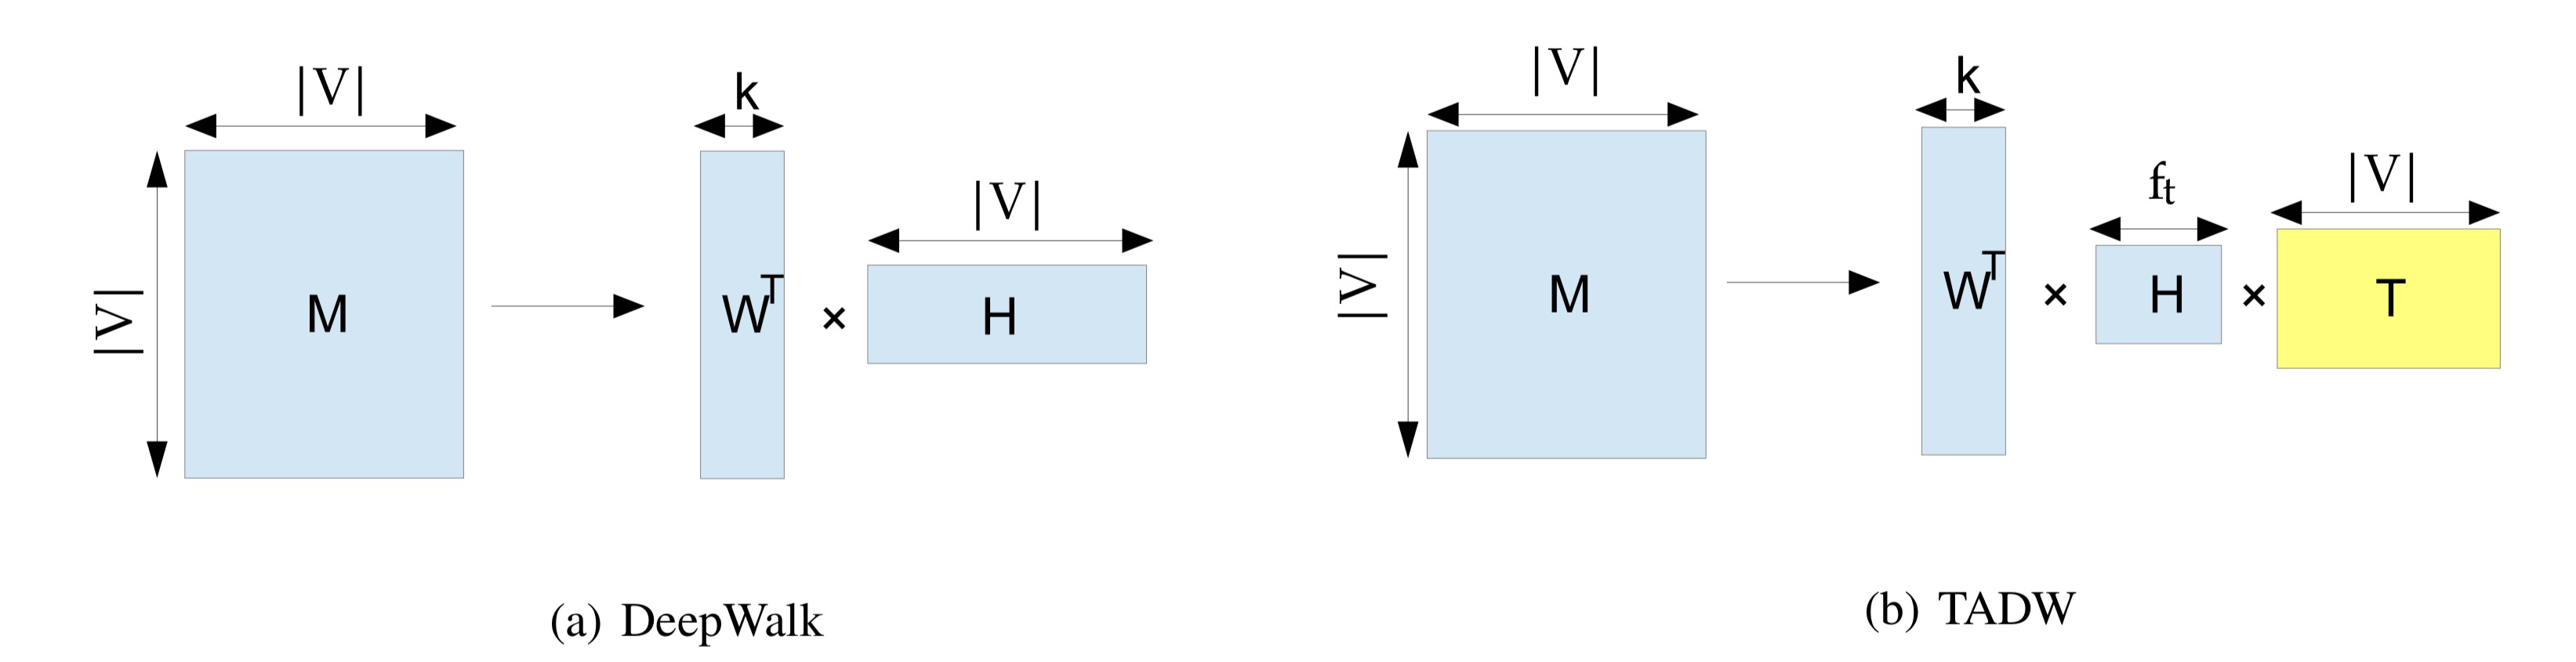
\includegraphics[width=5in]{figures/tadw.png}}
	\caption{DeepWalk和TADW的对比}\label{tadw}
\end{figure}


\section{增量学习}
现实的应用中,数据往往是以不断加入的。大型的社交网络中时刻都有节点的新增和边的增删,电商平台的交易数据也是在时刻更新积累。在动态变化场景中,频繁重新训练机器学习是非常浪费资源的。增量学习的思想是利用离线训练好的模型对新增数据进行学习和预测,省去重新批量式学习的过程。对于增量学习,文献\cite{zhong2017survey}中将分类增量学习分成三类:样本增量学习,特征增量学习和类别增量学习。大部分的增量场景集中在样本增量学习,同样的这一部分的研究文献和研究成果相较之下也比较多,其中一系列样本增量学习的算法是以随机梯度下降为原型进行优化,包括FOBOS算法,RDA算法和FTRL算法。下面将着重介绍其中的FOBOS算法。
 \begin{figure}[!ht]
	\centering
	{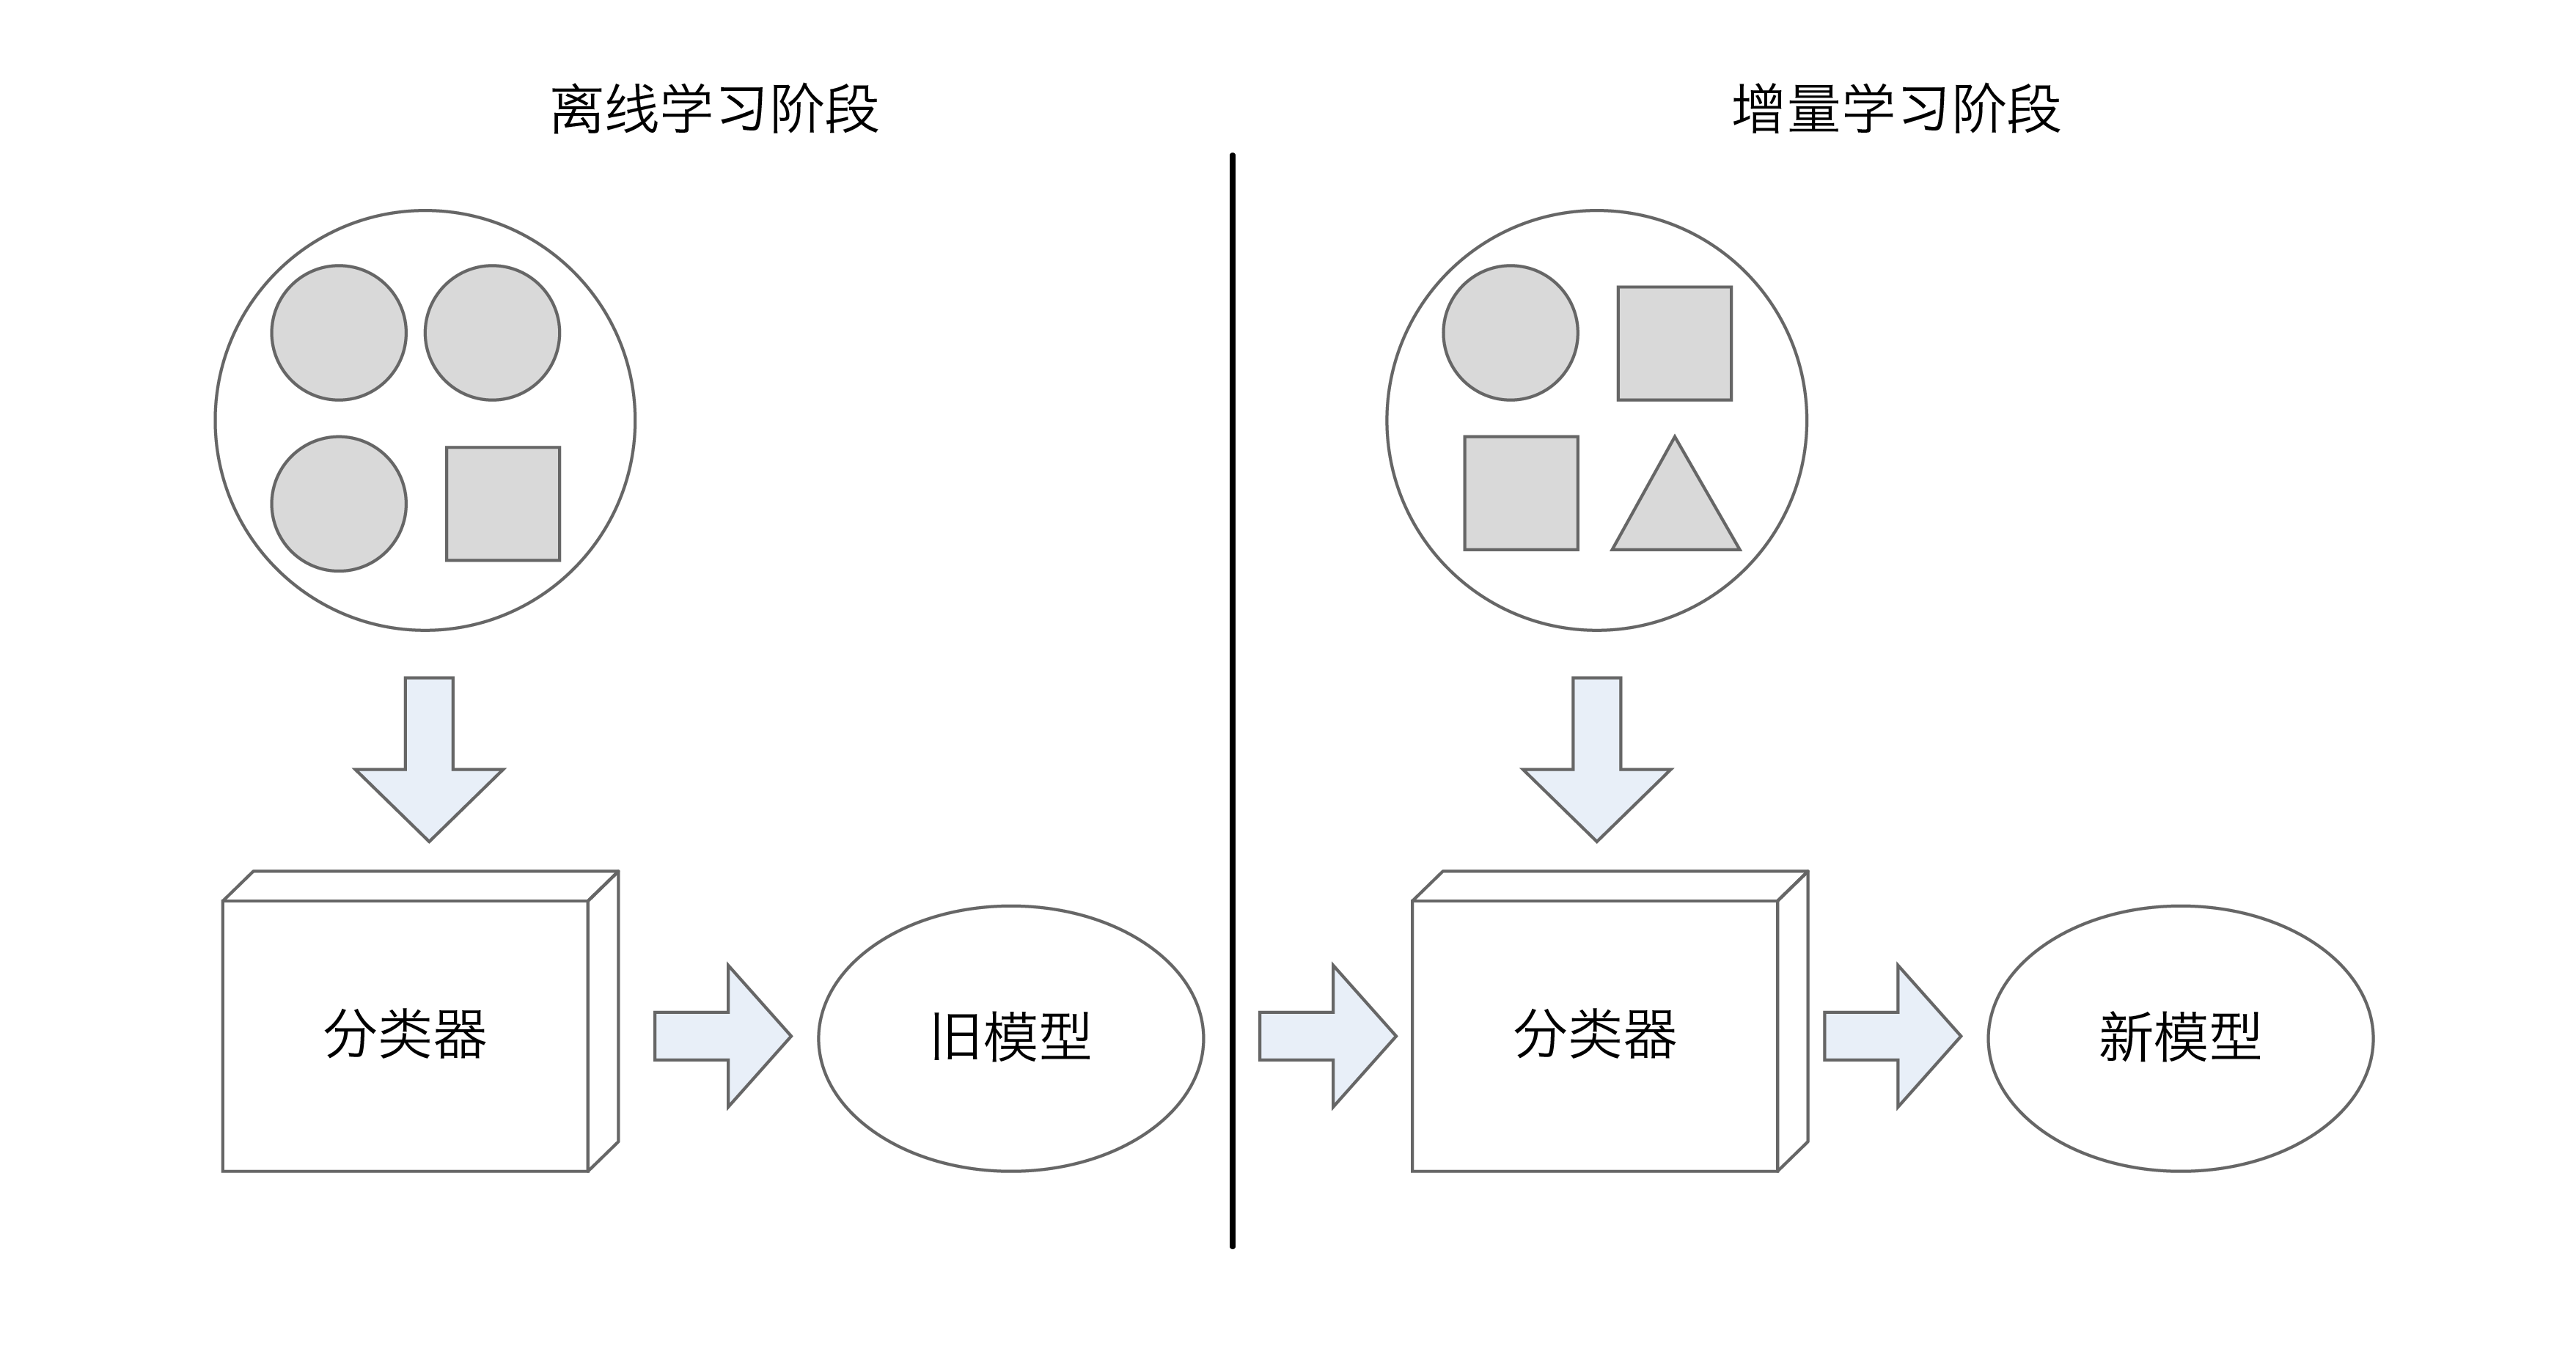
\includegraphics[width=5in]{figures/incremental_struct.png}}
	\caption{增量学习流程示意图}
\end{figure}

\subsection{FOBOS算法}
在应对在线数据流时,批量模式的算法会浪费大量资源,大部分增量学习的算法涌现。一部分增量算法在处理带非光滑正则项的凸优化问题时会出现问题,无法出现真正的稀疏解。对于带正则的无约束优化问题:
\begin{equation}
	\min_w \sum_{i-1}^{n}L(w,z_i) +\lambda|w|_1
\end{equation}
最常用的求解方法为梯度下降法,即令$w_{t+1} = w_t - \eta 
\nabla f(w_t)$,根据不同的要求可采用全局梯度下降、批量梯度下降或随机梯度下降(Stochastic Gradient Descent,SGD)。其中,随机梯度下降可以用于数据流场景下对优化问题进行求解;另外一种方式在线梯度下降(Online Gradient Descent, OGD)\cite{zinkevich2003online}也被用在这个场景,其参数更新方式为:
\begin{equation}
	w_{t+1} = \Pi_{\mathcal{H}}(w_t - \eta 
	\nabla f(w_t))
\end{equation}
其中算子$\Pi_{\mathcal{H}}(w)$是将向量$w$投影到离$w$最近且在假设空间$\mathcal{H}$中的向量。

随机梯度下降和在线梯度下降在实际应用中会存在两个问题:一方面,在加入了L1正则情况下,通过简单的梯度下降方式也很难得到稀疏解;另一方面,在部分不可微点无法利用次梯度进行迭代求解。为优化简单梯度下降,FOBOS算法将每一次的迭代过程分解成两步,包括一个梯度下降迭代和一个最优化过程:
\begin{equation}
\begin{aligned}
w_{t+\frac{1}{2}} = w_t -\eta_t 
\nabla f(w_t) \\
\min \quad \frac{1}{2}|w_t-w_{t+\frac{1}{2}}|^2 + \eta_{t+\frac{1}{2}}r(w_t)
\end{aligned}
\end{equation}
其中$r(w)$表示正则化函数,通过这种优化使得FOBOS算法获得的解与临时解$w_{t+\frac{1}{2}}$相近,同时使得学习到的参数更加具有稀疏性。FOBOS算法在梯度下降方法中所得解具有较好的稀疏,且具有不错的精度。之后发表的RDA算法能在精度和稀疏性之间做更好的平衡,FTRL算法更是结合了这两者的优点,具有不错的精度和稀疏性,在这里不再赘述。



%%%%%%%%%%%%%%%%%%%%%%%%%%%%%%%%%%%%%%%
%---------------------------------------     本章小结     ----------------------------------------%
%%%%%%%%%%%%%%%%%%%%%%%%%%%%%%%%%%%%%%%


\section{本章小结}
本章对论文中相关理论和算法进行了总结综述。主要分成三个方面。1.图表征算法的分类介绍。主要从接近度的概念对已有算法进行分类,其中从保留网络结构的一阶接近度算法中介绍了拉普拉斯特征映射算法LE;从保留一阶和二阶接近度的算法中介绍了LINE算法;在保留高阶接近度的算法中,介绍了采用随机游走的DeepWalk算法,分析并对比不同接近度在精度和复杂度上的差异。2.属性图网络表征的算法介绍,考虑到网络中节点包含丰富的文本属性,介绍了结合节点文本属性信息的TADW算法。3.增量学习的算法介绍,阐述现实场景对增量学习的需求,介绍了基于梯度下降方式优化的FOBOS算法,在精度和参数稀疏性上具有良好的表现。这三个部分的介绍将为后文算法的设计提供借鉴的思路。





	